\documentclass[12pt,a4paper]{article}
\usepackage{amsmath,amssymb,amsthm,epsf, graphicx, rotating}
\usepackage{fancyhdr}
\usepackage{subfig}
\usepackage{float}
\graphicspath{ {./images/} }

\pagestyle{empty}
\setlength{\parindent}{0pt}
\setlength{\textwidth}{6.5in}
\setlength{\oddsidemargin}{0in}
\addtolength{\textheight}{1in}

\renewcommand\theenumi{\alph{enumi}}
\renewcommand\labelenumi{(\theenumi)}

\newcommand{\Z}{\mathbb{Z}}
\newcommand{\F}{\mathbb{F}}
\newcommand{\R}{\mathbb{R}}
\newcommand{\C}{\mathbb{C}}
\newcommand{\N}{\mathbb{N}}
\renewcommand\vec{\mathbf}

\pagestyle{fancy}
\fancyhf{}
\fancyhead[LE, RO]{Ryan Liu}

\theoremstyle{definition}
\newtheorem{problem}{}

\author{Ryan Liu}
\title{MATH 442 Homework 10}
\begin{document}

\begin{center}
{\huge MATH 442 \par}
{\Large Homework  10  \par}
{\normalsize Name: Ryan Zhuo Lun Liu \par}
{\normalsize Student Number: 30328141 \par}
{\normalsize Collaborator: Robert Benjamin Lang \par}
\end{center}

\begin{problem} \underline{Answer:}
\begin{proof} The statement, $\tau(G) = \tau(G - e) + \tau(G/e)$ will be proved directly. \\

Consider a graph $G = (V, E)$ and an edge $e \in E$. When considering $\tau(G)$ in regards to $e$, we can represent $\tau(G)$ as as the number of spanning trees of $G$ that must not include $e$ and the number of spanning trees of $G$ that must include $e$. \\

Of course, $\tau(G - e)$ is the number of spanning trees of $G$ that must not include $e$. Now consider $G/e$, and observe that any spanning tree of $G/e$ can be expanded to include $e$. Thus, $\tau(G/e)$ is the number of spanning trees of $G$ that must include $e$. \\

Hence, $\tau(G) = \tau(G - e) + \tau(G/e)$.
\end{proof}
\end{problem}

\begin{problem} \underline{Answer:}
\begin{proof}
For both graphs, there are 60 non-isomorphic ways to label the graphs. \\

For the graph on the left, we first pick top most vertex and see that there are $\binom{5}{1}$ ways to label it. Next, we can look at the leftover square by itself, and see that the interesting vertices are now the two upper vertices as they were connected to the top most vertex. Since there are 4 labels remaining, there are $\binom{4}{2}$ ways to label it. For the remaining two, once you pick one, the other one just takes the last one and thus is just $\binom{2}{1}$. \\

Hence, there are $\binom{5}{1}\binom{4}{2}\binom{2}{1} = 60$ non-isomorphic ways to label this graph. \\

We can apply a similar technique for the second graph and pick the central vertex and see that there are still $\binom{5}{1}$ ways to label it. Observe that the remaining graph has one vertex of degree 0 (if you remove the edges related to the central vertex). We pick this as our next interesting vertex, and there are $\binom{4}{1}$ ways to label it. The remaining graph looks familiar to us, as it is one of the graphs we went over in class, and can represented by $\binom{3}{1}$. \\

Hence, there are $\binom{5}{1}\binom{4}{1}\binom{3}{1} = 60$ non-isomorphic ways to label this graph.
\end{proof}
\end{problem}

\begin{problem} \underline{Answer:}
\begin{proof} 
The Pr\"ufer Sequence associated with the given graph in $a)$ is ${5, 2, 2, 6, 2, 2}$. \\

The graph associated with the given sequence in $b)$ is: 
\begin{figure}[H]
    \centering
    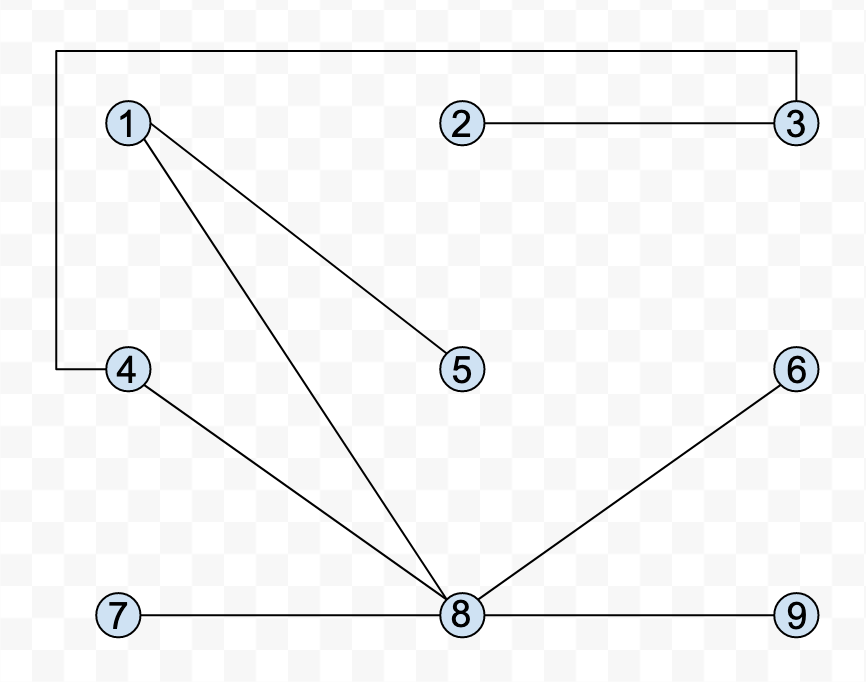
\includegraphics[scale=0.5]{q3.png}
    \caption{Q3}
    \label{fig:my_label}
\end{figure}
\end{proof}
\end{problem}

\begin{problem} \underline{Answer:}
\begin{proof} 
We will prove the statement, a vertex in a labelled tree $T$ has degree $k$ iff its label appears $k - 1$ times in the Pr\"ufer sequence of the tree. \\

$\rightarrow$ Consider a vertex $v$ that has degree $k$. Following the encoding algorithm, if $v$ is a leaf, then it will not be included in the Pr\"ufer sequence, and it follows the formula as $1 - 1 = 0$. \\

If $v$ is not a leaf, then we remove leaves from $T$ until we have 2 vertices remaining. Consider this process in regards to $v$, and we see that once we removed $k - 1$ vertices, $v$ becomes a leaf. Either $v$ gets removed and the vertex $u$ adjacent to $v$ gets put into the sequence or we've reached the end of the encoding algorithm and $v$ is one of 2 vertices not removed from $T$.\\

$\leftarrow$ Consider a label $x$ that appears $k - 1$ times. Following the decoding algorithm, we first start at a vertex whose label is not in the sequence, and that cannot be $v$ as its label, $x$, appears $k - 1$ times. Since $x$ appears $k - 1$ times, there are $k - 1$ vertices adjacent to $v$ in $T$. \\

Observe that once we have removed $x$ from the Pr\"ufer sequence, we have two cases. Either there are more numbers in the sequence to be removed or $x$ was the last label to be removed. In the first case, vertex $v$, which is the vertex represented by label $x$, is connected to a vertex $u$, labelled by $y$ and $v$ has degree $k$. In the second case, $x$ is one of the 2 remaining labels whose vertices should be joined together as indicated by the decoding algorithm, and $v$ has degree $k$. 
\end{proof}
\end{problem}

\begin{problem} \underline{Answer:}
\begin{proof} 
Consider a tree $T$ with the given configuration, and we see that there are $8$ vertices not specified. We will consider the "best" case, where they are all leaves, and thus each have a degree of $1$. The sum of degrees is then $5 + 4 + 4 + 2 + 8 = 23$. \\

We also know that any tree $G$ with $n$ vertices has $n - 1$ edges, or there is a cycle. Our configuration gave us 12 vertices, giving us 11 edges. We also know that the sum of degrees of any graph is twice the number of edges, and thus for 12 vertices, the sum should be 22. However, we had 23 above and we arrive at a contradiction. 
\end{proof}
\end{problem}

\begin{problem} \underline{Answer:}
\begin{proof} 
Given the configuration, we see that there is only one possible graph, shown in figure 2

\begin{figure}[H]
    \centering
    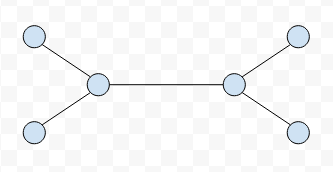
\includegraphics[scale=0.5]{q6.png}
    \caption{Q6}
    \label{fig:my_label}
\end{figure}

We know that we cannot have a tree with every vertex of degree 1. Since we are only allowed degrees 1 or 3, at least one vertex is of degree 3, and we see that if all three vertices are of degree 1, we only have four vertices out of the required six. However, if one of the three also has degree 3, we have exactly six vertices, and every vertex has degree 1 or 3. \\

This configuration gives us 90 non-isomorphic ways to label the graph. Let's pick the interesting vertices, namely the two central vertices of degree 3. We see that if we were to pick one and label it, there are $\binom{6}{1}$ ways, leaving the other one with $\binom{5}{1}$. \\

Now let's consider the 4 leaves, and observe the symmetry. Not only can we swap the left and right sections, we can also swap between each section individually. This implies that the number of non-isomorphic ways to label the 4 leaves is the number of ways to split the four remaining labels into two graphs, giving us $\frac{\binom{4}{2}}{2}$. \\

Combining the expressions gives us $\binom{6}{1}\binom{5}{1}\binom{4}{2}(\frac{1}{2}) = 90$.
\end{proof}
\end{problem}
\end{document}
